\section{Applying different filters to the image}\label{P2}

Three distinct filters, namely the moving average filter, the low-pass Gaussian filter, and the median filter, have been developed specifically for application to the images. Initially, the moving average filter is conceived of and developed. Three-by-three and seven-by-seven pixel filters are built in order to evaluate the impact of the moving average filter size. Figure 2 illustrates the form of the 7*7 filter that is being processed.


\begin{figure} [ht]
    \centering
    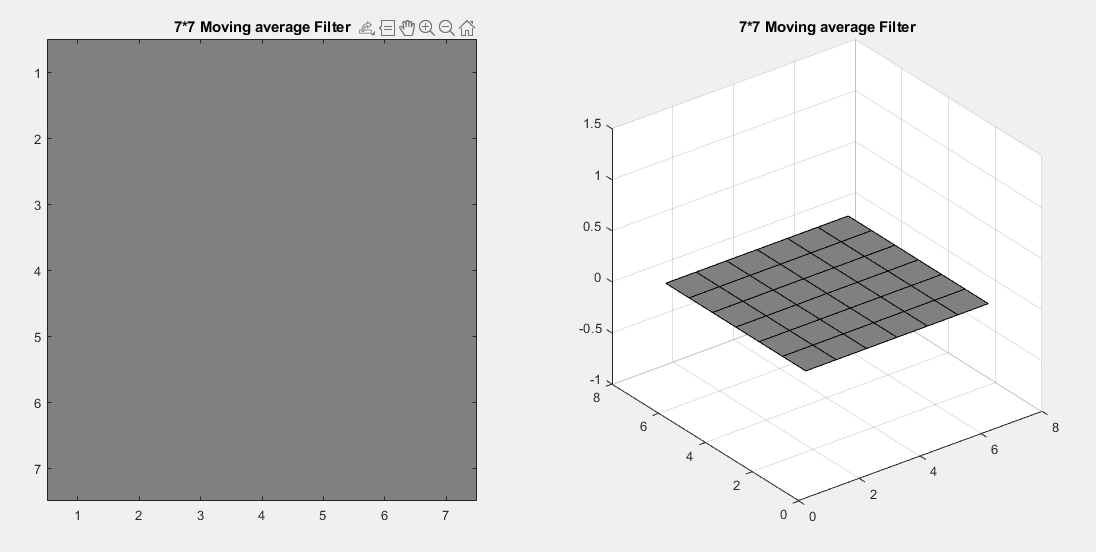
\includegraphics[width = \textwidth]{Resources/Avg_filter.png}
    \caption{Moving average filter with 7*7 pixels}
    \label{fig:ApplyingFilters}
\end{figure}

Following the application of these two moving average filters to the image that contains Gaussian noise, it is possible to observe, on the basis of the plots presented in Figure 3, that the 3*3 pixels filter eliminates a portion of the noise associated with the image. It should be noted, however, that the image still contains a significant amount of noise. There is a significant reduction in the amount of noise in the picture when the size of the filter is increased to 7 by 7. Unfortunately, some of the picture's features are lost, and the picture itself gets hazy, which is not something that is desirable for some tasks. In this section, a function is built to plot the figures in order to reduce the amount of code that is currently being composed. In order to draw the plot of the image and its histogram, this function obtains the name of the image, the name of the noise, the name of the filter, and the size of the filter. 
Salt and pepper noise is next applied to the image, and then the moving average filters are applied to the image. It is clear from the findings presented in Figure 4 that the moving average filters are not effective in removing the salt and pepper noise from the data. There is not much of an impact that the image filter with 3*3 pixels has on the picture because the picture is still entirely noisy throughout. On the other hand, the picture becomes indistinct when the 7*7 pixels moving average filter is applied there. It should be brought to your attention that even when the 7*7 filter is utilized, a significant amount of noise can still be observed.

\begin{figure} [ht]
    \centering
    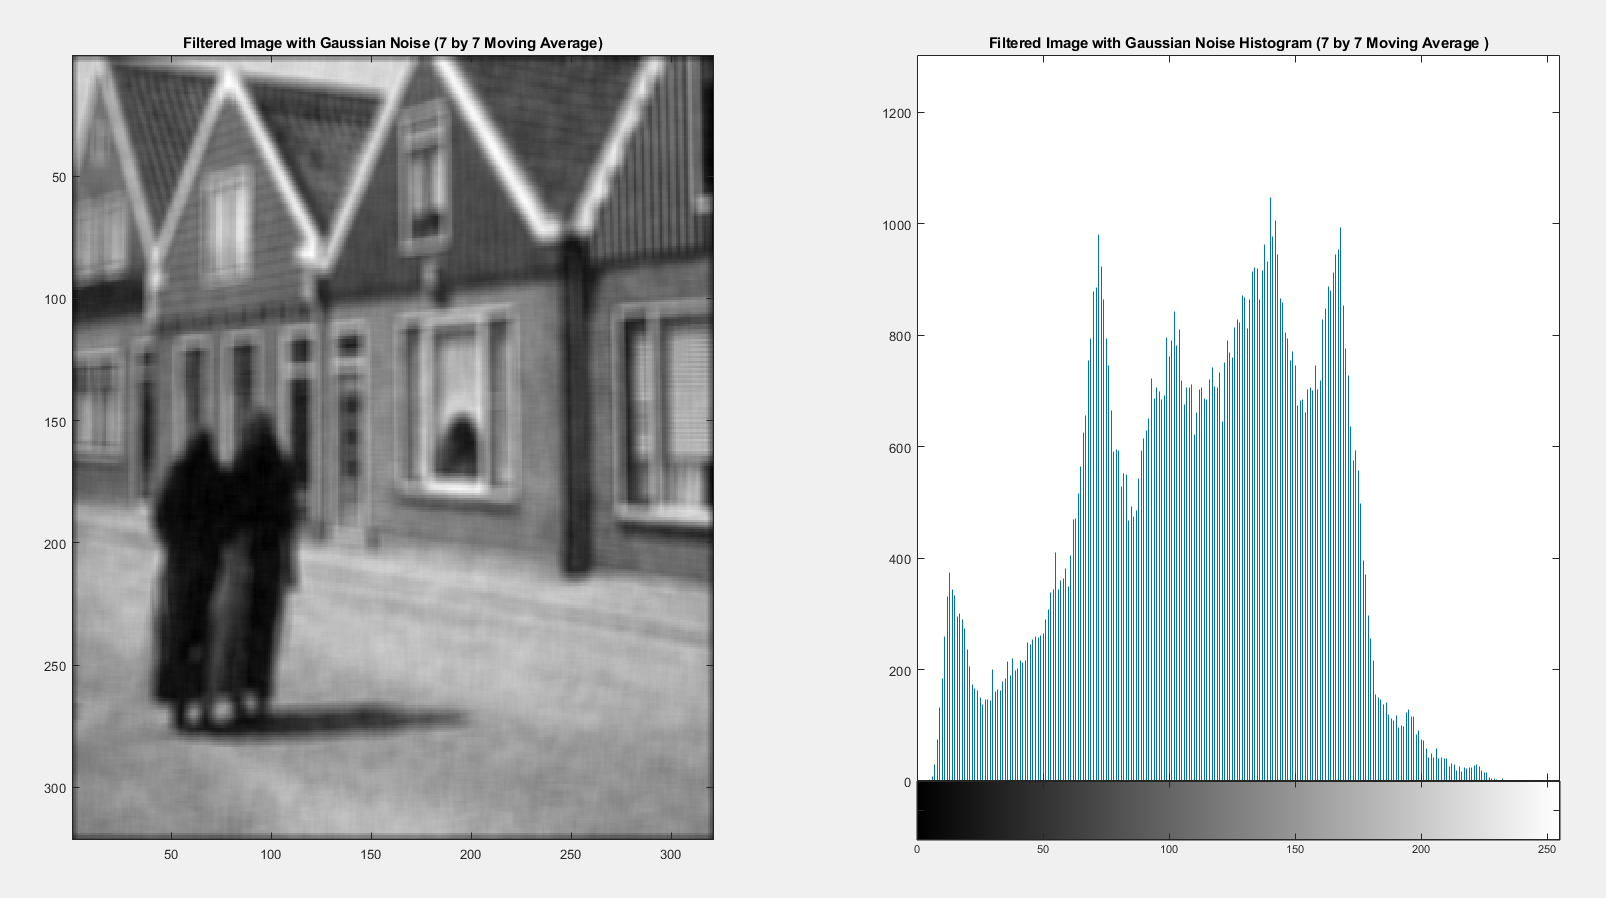
\includegraphics[scale = 1, angle=0]{Resources/Image with Gaussian noise filter by a moving average filter.png}
    \caption{Image with Gaussian noise filter by a moving average filter with 7*7 pixels}
    \label{fig:ApplyingFilters}
\end{figure}

\newpage

\begin{figure} [ht]
    \centering
    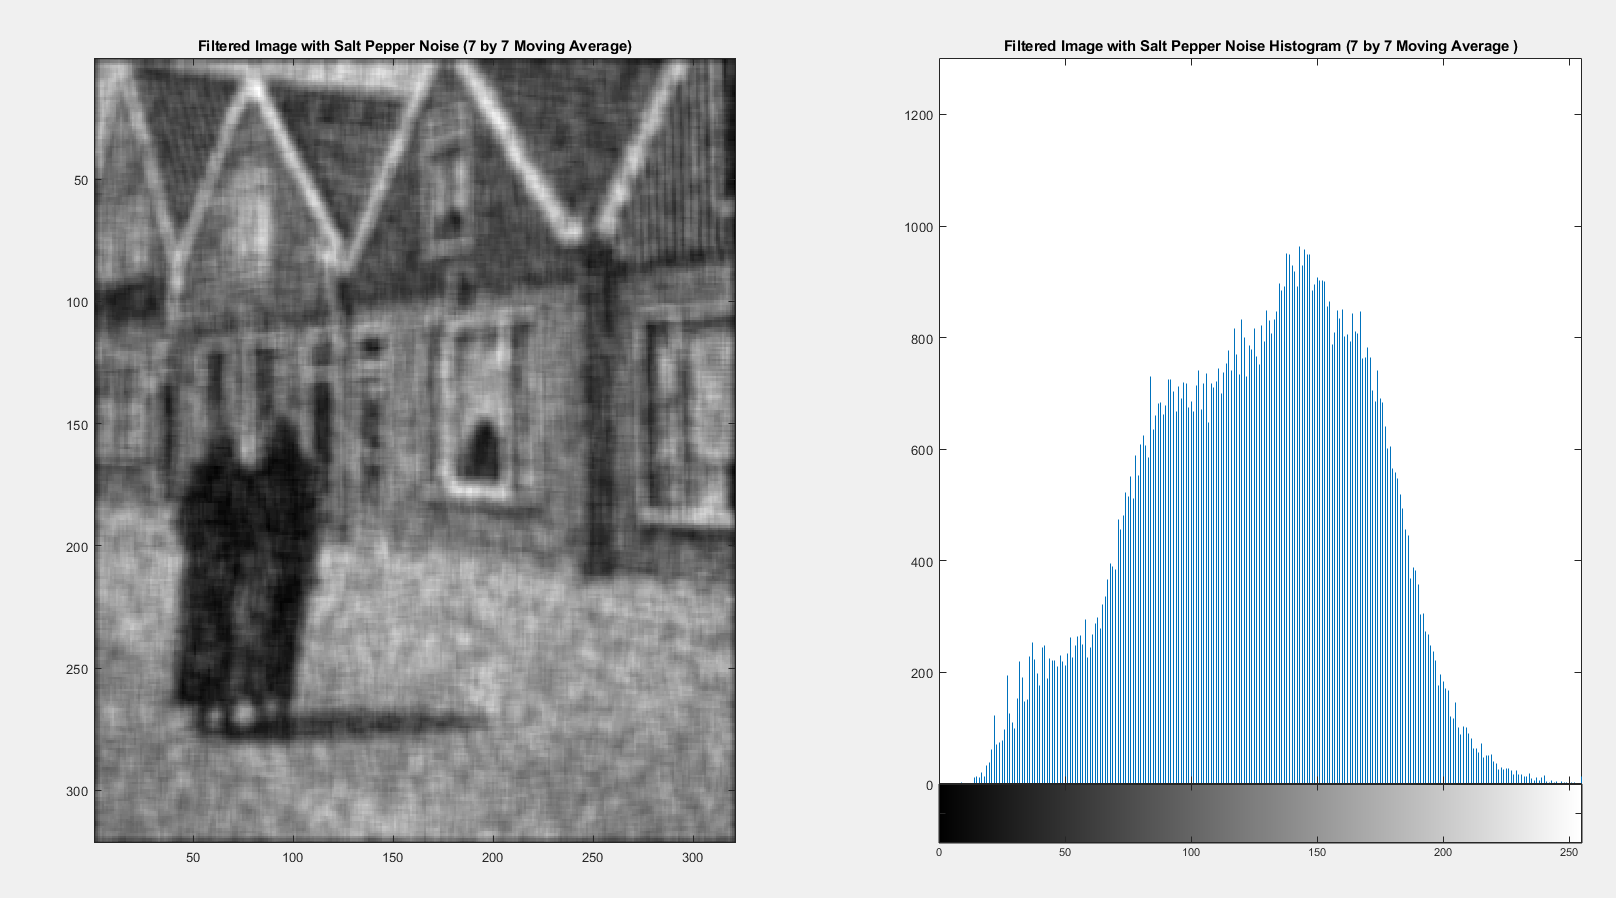
\includegraphics[scale = 1, angle=0]{Resources/Image with Salt & Pepper noise filter by moving average filter.png}
    \caption{Image with Salt \& Pepper noise filter by moving average filter with 7*7 pixels}
    \label{fig:ApplyingFilters}
\end{figure}

As a result of the fact that low-pass Gaussian filters give greater weight to the central pixel as opposed to giving the same weight to all of the neighborhood pixels, it is anticipated that these filters will demonstrate a higher level of accuracy in contrast to moving average filters. The creation of low-pass Gaussian filters with 3*3 and 7*7 pixels is demonstrated in Figure 5, with the 7*7 filter being the one that is most visible.

\begin{figure} [ht]
    \centering
    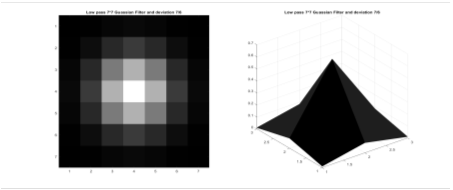
\includegraphics[scale = 1, angle=0]{Resources/Low pass Gaussian filter.png}
    \caption{Low pass Gaussian filter with 7*7 pixel size}
    \label{fig:ApplyingFilters}
\end{figure}

The use of both 3*3 and 7*7 low pass Gaussian filters on the image that contains Gaussian noise reveals, as shown in Figure 6, that this filter has been successful in reducing the noise to a level that is acceptable. When compared to the moving average filter of the same size, the 7*7 filter is able to totally eliminate the majority of the noise, and despite the fact that the picture becomes slightly blurry, it is still able to display the correct features of the image.
When applying the low-pass Gaussian filters that were constructed to the image that had Salt \& Pepper noise, the identical difficulty and problem that the moving average filter presented is encountered. To obtain a new value for that filter, it takes the value of the central pixel and the values of some nearby pixels and adds them together. This is based on the concept of the Gaussian filter. Within the context of this summing, however, it gives the central pixel a greater weight. This approach is not capable of effectively removing this type of noise because the salt and pepper noise adds some pixels to the image that are entirely white and black. These pixels will continue to be there even after the filter has been applied, regardless of whether or not the filter size is increased. In spite of the fact that the size was increased, it is evident from Figure 7 that the noise is still present, and the picture also loses some of its details. 

After everything is said and done, two median filters with pixel widths of 3*3 and 7*7 are constructed and applied to images that contain Gaussian noise as well as Salt \& pepper noise. These filters are displayed in Figure 8 and Figure 9, respectively. When it comes to removing salt and pepper noise, this particular type of filter performs far better than the moving average and Gaussian filters, as demonstrated in Figure 9. In comparison to the values of the pixels that are adjacent to it, median filters select the pixel value that has the median intensity. Both the intensity of the salt and pepper noise pixels is either too high or too small. As a consequence of this, the noise pixels are regarded as outliers on the basis of their intensity value, and a final image that is appropriately composed is produced. The one and only issue with this is that it does not take into account the minute elements of the photo, such as the thin and small lines that are on the walls. This may be owing to the fact that the intensity value of these lines may be considered to be outliers and noise in this particular instance. It is possible that increasing the size of this filter will result in the loss of further minute details, leaving just the primary details of the picture, such as the shape of the houses and the borders of the people to be preserved.  

\newpage

\begin{figure} [ht]
    \centering
    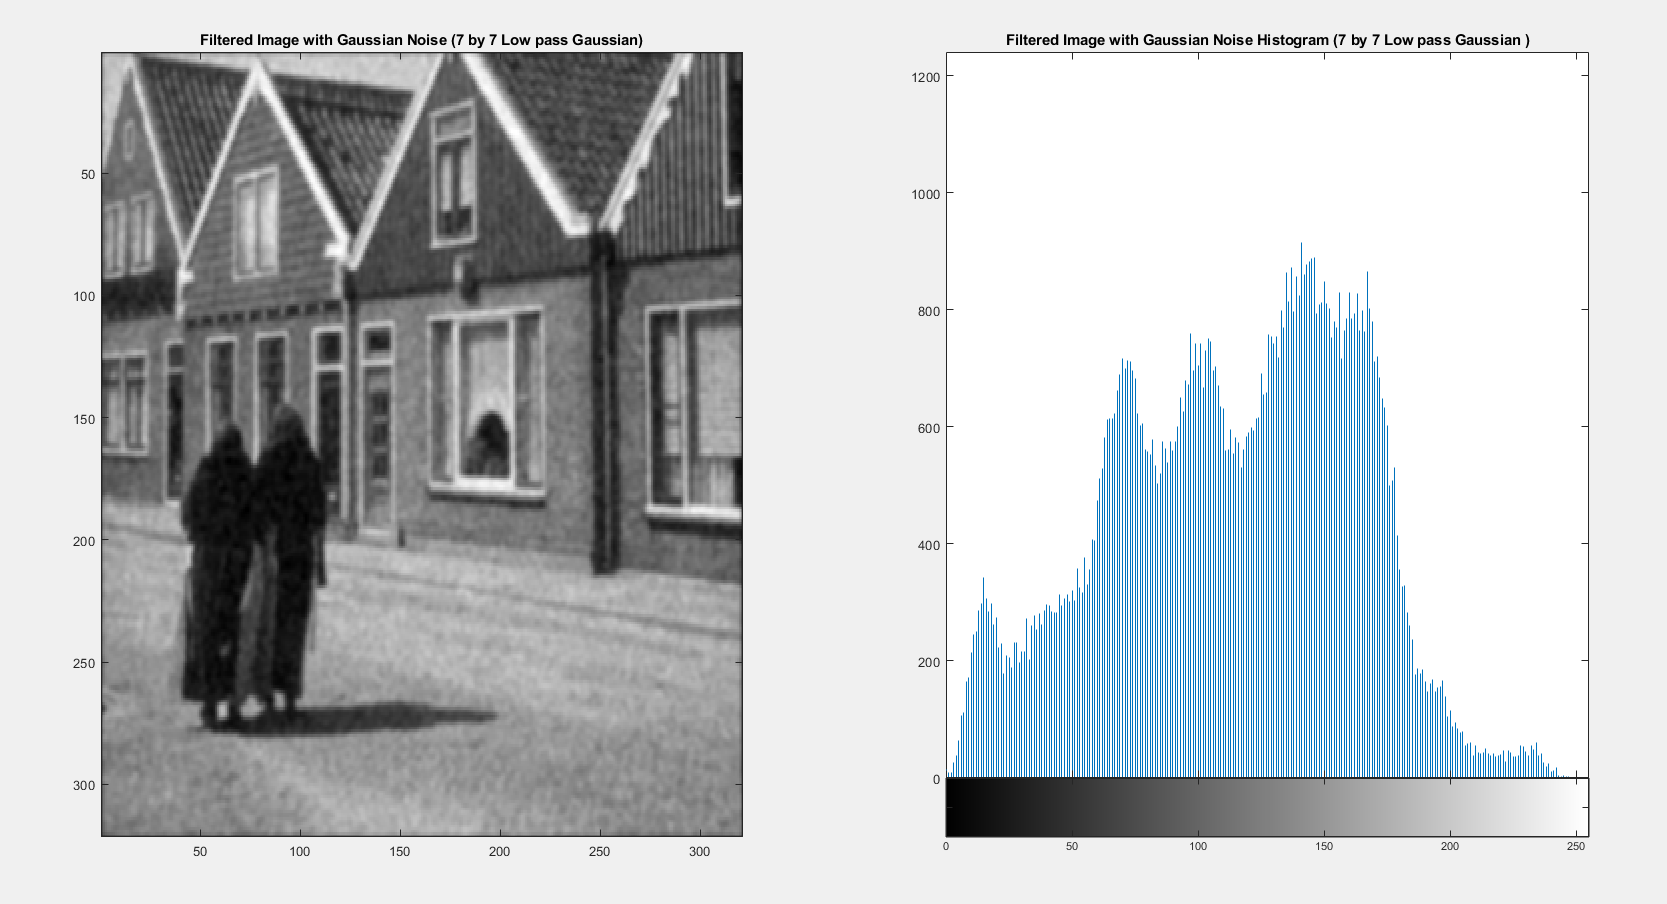
\includegraphics[scale = 1, angle=0]{Resources/Image with Gaussian noise filtered by low-pass Gaussian filter.png}
    \caption{Image with Gaussian noise filtered by low-pass Gaussian filter with 7*7 pixels}
    \label{fig:ApplyingFilters}
\end{figure}

\begin{figure} [ht]
    \centering
    \begin{subfigure}{0.4\textwidth}
        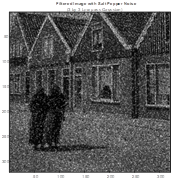
\includegraphics[width=\textwidth]{Resources/F7-a.png}
        \caption{}
        \label{fig:first}
    \end{subfigure}
    \hfill
    \begin{subfigure}{0.4\textwidth}
        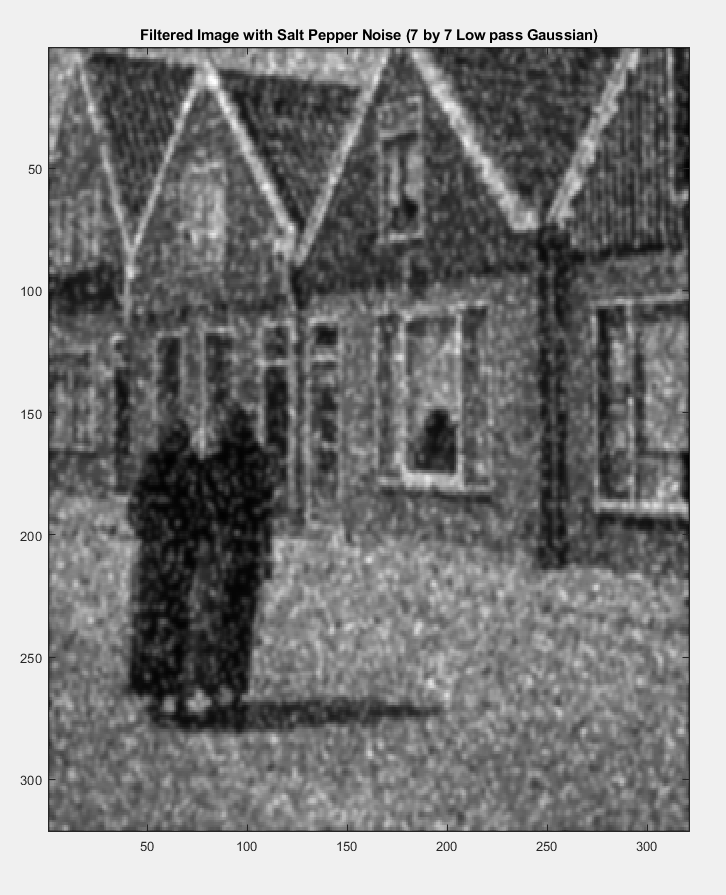
\includegraphics[width=\textwidth]{Resources/F7-b.png}
        \caption{}
        \label{fig:Second}
    \end{subfigure}
    \caption{Image with Salt \& Pepper noise filtered by low-pass Gaussian filter with (a) 3*3, and (b) 7*7 pixels}
    \label{fig:ApplyingFilters}
\end{figure}


\begin{figure}
    \centering
    \begin{subfigure}{0.4\textwidth}
        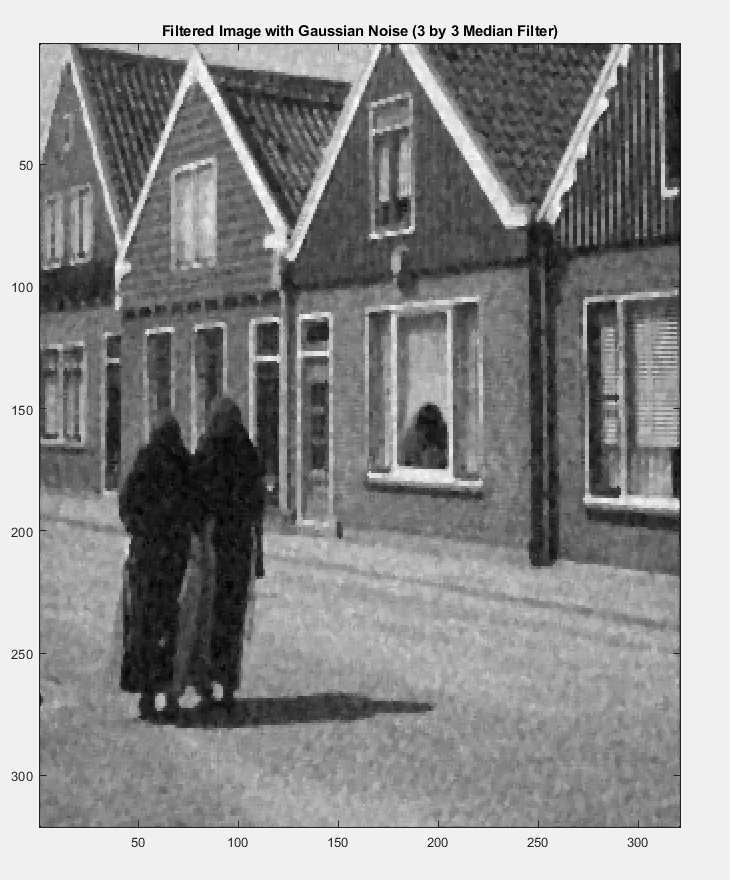
\includegraphics[width=\textwidth]{Resources/F8-a.png}
        \caption{}
        \label{fig:first}
    \end{subfigure}
    \hfill
    \begin{subfigure}{0.4\textwidth}
        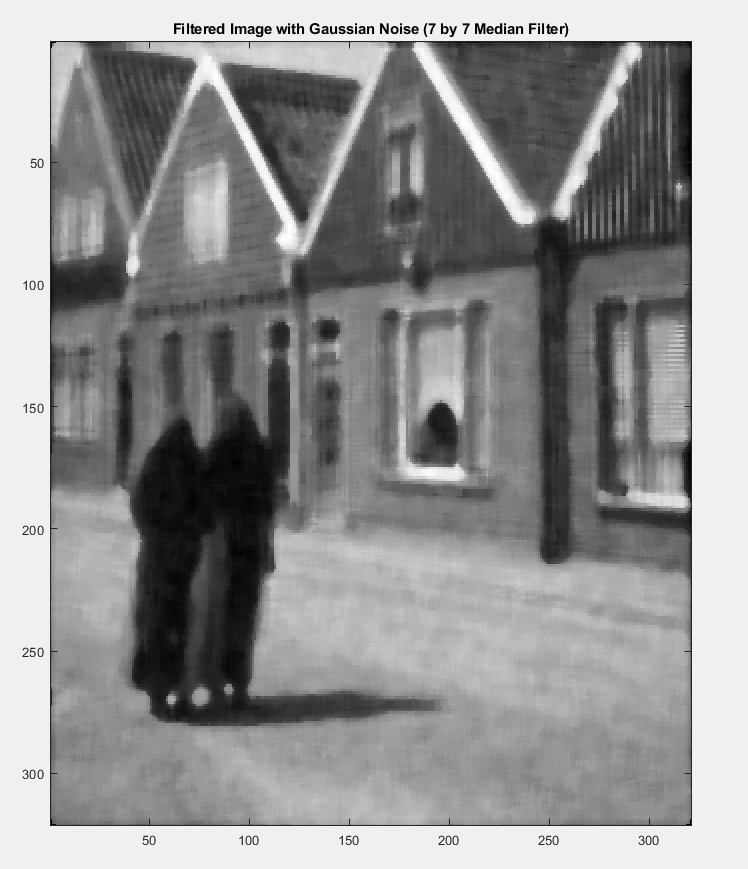
\includegraphics[width=\textwidth]{Resources/F8-b.png}
        \caption{}
        \label{fig:Second}
    \end{subfigure}
    \caption{Image with Gaussian noise filtered by Median filter with (a) 3*3, and (b) 7*7 pixels}
    \label{fig:ApplyingFilters}
\end{figure}

\begin{figure}
    \centering
    \begin{subfigure}{0.4\textwidth}
        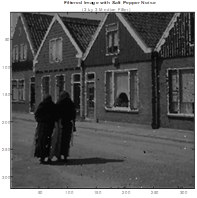
\includegraphics[width=\textwidth]{Resources/F9-a.png}
        \caption{}
        \label{fig:first}
    \end{subfigure}
    \hfill
    \begin{subfigure}{0.4\textwidth}
        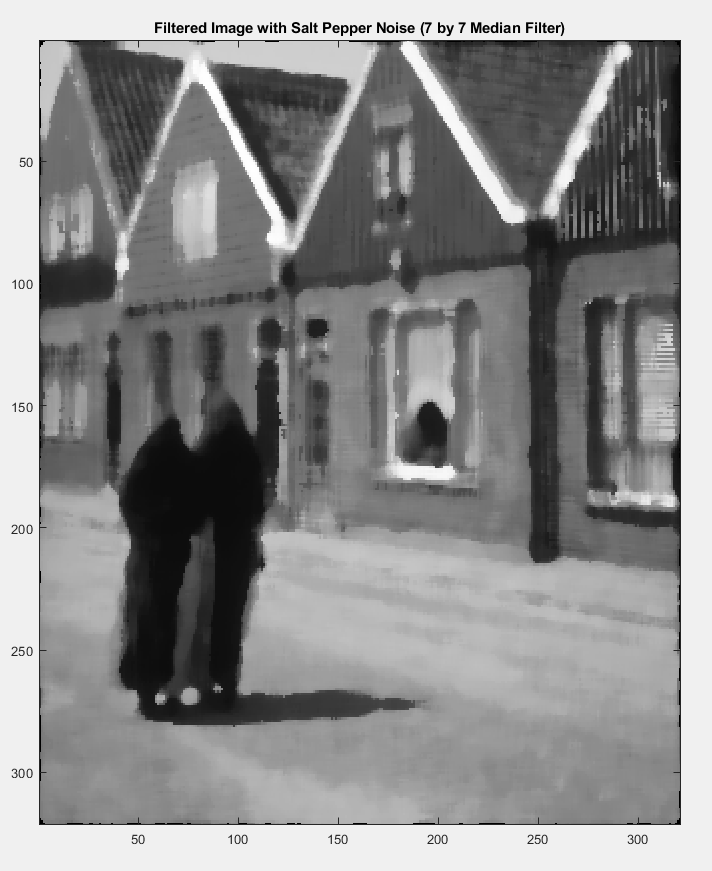
\includegraphics[width=\textwidth]{Resources/F9-b.png}
        \caption{}
        \label{fig:Second}
    \end{subfigure}
    \caption{Image with Salt \& pepper noise filtered by Median filter with (a) 3*3, and (b) 7*7 pixels}
    \label{fig:ApplyingFilters}
\end{figure}